\chapter{Comparative Models}

\section{Introduction to Baseline Models}

To provide context for the robustness and verification of the Liquid Neural Network (LNN), we benchmark its performance against three established neural architectures: the Temporal Convolutional Network (TCN), the Long Short-Term Memory (LSTM) network, and the Transformer model. All models are trained on the same trajectory prediction task, using identical datasets, normalisation, loss functions, and training schedules as the LNN.

The selection of these baselines is motivated by their contrasting inductive biases and proven success in modelling sequential data. The LSTM is a recurrent architecture that introduces gating mechanisms and persistent internal states, enabling it to model long-range temporal dependencies through iterative state updates. The TCN, however, uses on dilated causal convolutions and fixed temporal receptive fields, making it structurally different from recurrent networks and well-suited for parallel computation. The transformer model is an attention-based architecture, which eliminates recurrence altogether, and dynamically weight input positions using self-attention mechanisms. It applies positional encodings to retain order information.

By evaluating the behaviour of these models under clean and adversarial conditions, we aim to identify both their predictive accuracy, and their robustness, sensitivity to perturbation, and qualitative output characteristics. These insights provide context for assessing the LNN in the following aspects:

\begin{itemize}
    \item \textbf{Temporal memory:} How effectively each model retains and processes sequential dependencies
    \item \textbf{Structural robustness:} The influence of architectural constraints on noise sensitivity
    \item \textbf{Gradient stability:} The relationship between loss geometry and adversarial vulnerability
\end{itemize}


\section{Temporal Convolutional Network (TCN)}

\subsection{Overview and Motivation}
The Temporal Convolutional Network (TCN) is a fully convolutional architecture designed for sequential data. Unlike RNN-based models, which process inputs recursively and maintain an internal hidden state, TCNs rely on 1D convolutions applied over the temporal axis. This allows for parallel computation and more stable gradients, particularly for long sequences.

TCN's use \textbf{dilated convolutions}, which expand the receptive field exponentially with depth while preserving causality. This makes them highly effective at modelling long-range dependencies without the vanishing gradient issues that often affect RNNs.

\subsection{Theoretical Background}
For a 1D input sequence $x \in \mathbb{R}^{T \times d}$, a dilated convolution with kernel $k$ and dilation factor $d$ is defined as:
\[
(y *_{d} k)(t) = \sum_{i=0}^{k-1} k(i) \cdot x(t - d \cdot i)
\]
This structure allows the model to observe wider contexts with fewer parameters and layers.

In practice, the TCN is constructed using \textbf{residual blocks} with stacked dilated convolutions, dropout, and skip connections to stabilise training. Zero-padding is used to ensure output length matches input length.

\subsection{Model Architecture}
The implemented TCN consists of 3 residual blocks, each with:
\begin{itemize}
    \item Two 1D convolutional layers with kernel size 3
    \item Dilation rates of 1, 2, and 4 respectively
    \item ReLU activations and dropout regularisation
    \item Optional 1x1 convolutions for matching input-output dimensions
\end{itemize}
An output convolution maps the final hidden representation to the desired 2D coordinate space.

\begin{lstlisting}[language=Python, caption={Simplified TCN architecture}]
class ResidualBlock(nn.Module):
    def __init__(self, in_channels, out_channels, kernel_size, dilation, dropout):
        ...
        self.conv1 = nn.Conv1d(..., dilation=dilation)
        self.conv2 = nn.Conv1d(..., dilation=dilation)

class TCN(nn.Module):
    def __init__(self, input_dim=2, hidden_channels=128, ...):
        self.tcn = nn.Sequential(*residual_blocks)
        self.output_layer = nn.Conv1d(hidden_channels, output_dim, 1)
\end{lstlisting}

\hl{PUT TCN INFEENCE EXAMPLE/ARCHITECTURE DIAGRAM HERE}


\begin{figure}[H]
    \centering
    \begin{tikzpicture}[scale=1, every node/.style={transform shape}]

        % Input
        \node[draw, rounded corners, minimum width=3.5cm, minimum height=1cm, fill=blue!10] (input) at (0, 0) {Input Sequence};

        % Residual Block 1
        \node[draw, rounded corners, minimum width=3.5cm, minimum height=1cm, fill=red!15] (res1) at (0, -1.5) {Residual Block (dil=1)};
        \draw[->, thick] (input) -- (res1);

        % Residual Block 2
        \node[draw, rounded corners, minimum width=3.5cm, minimum height=1cm, fill=red!20] (res2) at (0, -3.0) {Residual Block (dil=2)};
        \draw[->, thick] (res1) -- (res2);

        % Residual Block 3
        \node[draw, rounded corners, minimum width=3.5cm, minimum height=1cm, fill=red!25] (res3) at (0, -4.5) {Residual Block (dil=4)};
        \draw[->, thick] (res2) -- (res3);

        % Output Conv
        \node[draw, rounded corners, minimum width=3.5cm, minimum height=1cm, fill=cyan!10] (out) at (0, -6.0) {1x1 Conv Output Layer};
        \draw[->, thick] (res3) -- (out);

        % Output
        \node[below=0.2cm of out] (final) {\textbf{Predicted Coordinates}};
        \draw[->, thick] (out) -- (final);

        % Label
        \node at (0, -7.2) {\textit{Stacked Dilated Residual Convolutions in the TCN}};
    \end{tikzpicture}
    \caption{Temporal Convolutional Network (TCN) architecture with 3 residual blocks and exponentially increasing dilation. Each block contains two dilated convolutions with dropout, ReLU, and optional skip connection.}
    \label{fig:tcn_architecture}
\end{figure}


\subsection{Training Configuration}
The TCN was trained on the same spiral dataset as the LNN, with identical batch size, learning rate, loss function (Smooth L1), and normalisation pipeline. The model was optimised using Adam and a learning rate scheduler that halved the rate every 500 steps.

\subsection{Performance and Behaviour}
The TCN demonstrated strong performance on the trajectory prediction task, converging more quickly than the LNN and producing smooth outputs even with a small receptive field. The use of dilated convolutions allowed the model to predict coordinated curvature without explicitly tracking hidden state over time.

\subsection{Design Considerations}
\begin{itemize}
    \item \textbf{Causality:} All convolutions were causal, ensuring no future information was used during prediction.
    \item \textbf{Parameter efficiency:} Despite having no recurrence, the TCN was able to model complex spirals with relatively few layers and a compact parameter set.
    \item \textbf{Regularisation:} Dropout was used within each block to avoid overfitting, as convolutional models tend to memorise local structures in small datasets.
\end{itemize}

Despite lacking the dynamic time constants of the LNN, the TCN proved to be a strong baseline in terms of speed, stability, and accuracy under clean conditions.


\section{Long Short-Term Memory Network (LSTM)}

\subsection{Background and Rationale}
The Long Short-Term Memory (LSTM) network is a popular recurrent neural architectures for sequential learning tasks. It was introduced to address the limitations of classical RNNs, particularly the vanishing and exploding gradient problems during backpropagation through time. The LSTM introduces gated memory units that regulate the flow of information over time.

Their ability to retain past information via internal cell states makes them well-suited for temporal tasks such as trajectory prediction.

\subsection{LSTM Cell Mechanics}
An LSTM cell maintains two internal states: a hidden state $h_t$ and a cell state $c_t$. The cell's behaviour is controlled by three gates:
\[
\begin{aligned}
f_t &= \sigma(W_f x_t + U_f h_{t-1} + b_f) \quad &\text{(forget gate)} \\
i_t &= \sigma(W_i x_t + U_i h_{t-1} + b_i) \quad &\text{(input gate)} \\
o_t &= \sigma(W_o x_t + U_o h_{t-1} + b_o) \quad &\text{(output gate)} \\
\tilde{c}_t &= \tanh(W_c x_t + U_c h_{t-1} + b_c) \quad &\text{(cell candidate)} \\
c_t &= f_t \odot c_{t-1} + i_t \odot \tilde{c}_t \\
h_t &= o_t \odot \tanh(c_t)
\end{aligned}
\]
These equations define how the LSTM updates its memory and hidden representations at each time step.

\subsection{Model Implementation}
In this project, the LSTM was implemented using PyTorch’s built-in \texttt{nn.LSTM} module. A two-layer LSTM was used, with 128 hidden units per layer. The final hidden state was passed through a linear projection layer to produce the 2D coordinate output.

\begin{lstlisting}[language=Python, caption={Simplified LSTM model structure}]
class LSTMModel(nn.Module):
    def __init__(self, input_dim=2, hidden_dim=128, num_layers=2, output_dim=2):
        self.lstm = nn.LSTM(input_dim, hidden_dim, num_layers, batch_first=True)
        self.output_layer = nn.Linear(hidden_dim, output_dim)

    def forward(self, x):
        out, _ = self.lstm(x)
        return self.output_layer(out)
\end{lstlisting}

\subsection{Training Configuration}
The LSTM was trained using the same dataset and preprocessing pipeline as the LNN and TCN. The Smooth L1 loss was used, and training was performed over 1000 epochs with a learning rate of 0.005. A step decay scheduler was applied halfway through training.

\subsection{Training Observations}
The LSTM showed stable training behaviour and low final validation loss. However, unlike the TCN and LNN, it exhibited slightly slower convergence. Its outputs were smooth and consistent, although it occasionally underfit regions with sharper curvature.

\hl{PUT LSTM INFEENCE EXAMPLE/ARCHITECTURE DIAGRAM HERE}

\begin{figure}[H]
    \centering
    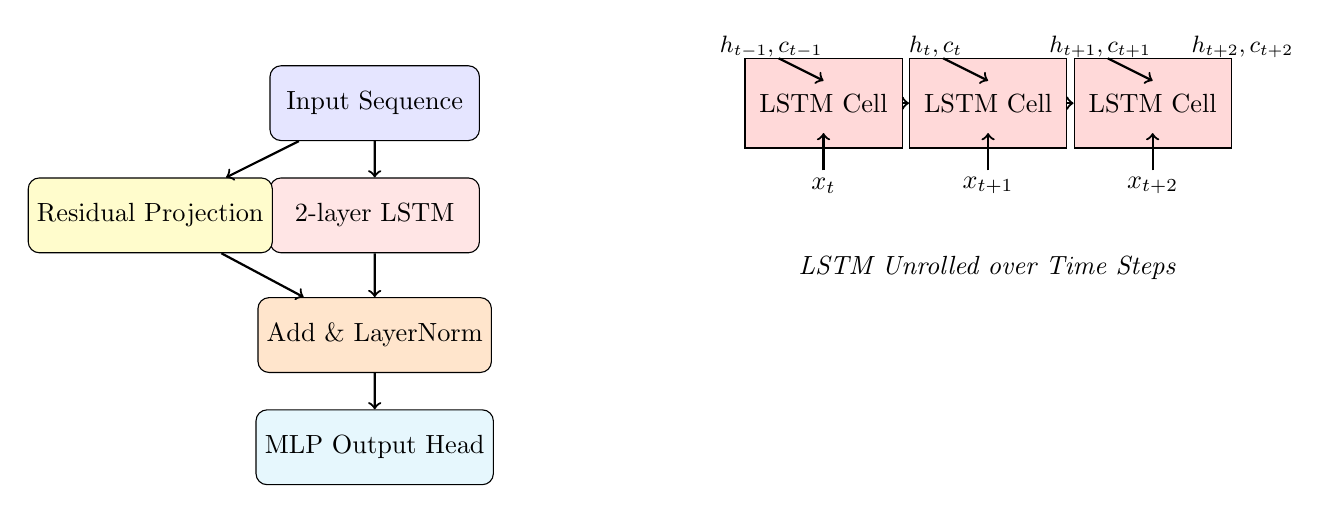
\begin{tikzpicture}[scale=0.95, every node/.style={transform shape}]

        % ------------------ High-level Architecture ------------------

        % Input
        \node[draw, rounded corners, minimum width=2.8cm, minimum height=1cm, fill=blue!10] (input) at (-5,0) {Input Sequence};

        % LSTM
        \node[draw, rounded corners, minimum width=2.8cm, minimum height=1cm, fill=red!10] (lstm) at (-5,-1.5) {2-layer LSTM};

        % Residual
        \node[draw, rounded corners, minimum width=2.8cm, minimum height=1cm, fill=yellow!20] (res) at (-8,-1.5) {Residual Projection};

        % Add + Norm
        \node[draw, rounded corners, minimum width=2.8cm, minimum height=1cm, fill=orange!20] (norm) at (-5,-3.1) {Add \& LayerNorm};

        % Output
        \node[draw, rounded corners, minimum width=2.8cm, minimum height=1cm, fill=cyan!10] (mlp) at (-5,-4.6) {MLP Output Head};

        % Arrows
        \draw[->, thick] (input) -- (lstm);
        \draw[->, thick] (input) -- (res);
        \draw[->, thick] (lstm) -- (norm);
        \draw[->, thick] (res) -- (norm);
        \draw[->, thick] (norm) -- (mlp);


        % ------------------ Unrolled LSTM ------------------

        \node[draw, minimum width=2.1cm, minimum height=1.2cm, fill=red!15] (cell1) at (1,0) {LSTM Cell};
        \node[draw, minimum width=2.1cm, minimum height=1.2cm, fill=red!15] (cell2) at (3.2,0) {LSTM Cell};
        \node[draw, minimum width=2.1cm, minimum height=1.2cm, fill=red!15] (cell3) at (5.4,0) {LSTM Cell};

        % Arrows
        \draw[->, thick] (cell1) -- (cell2);
        \draw[->, thick] (cell2) -- (cell3);

        % Inputs
        \node at (1,-1.1) {$x_t$};
        \node at (3.2,-1.1) {$x_{t+1}$};
        \node at (5.4,-1.1) {$x_{t+2}$};

        \draw[->, thick] (1,-0.9) -- (1,-0.4);
        \draw[->, thick] (3.2,-0.9) -- (3.2,-0.4);
        \draw[->, thick] (5.4,-0.9) -- (5.4,-0.4);

        % States
        \node at (0.3,0.75) {\small $h_{t-1}, c_{t-1}$};
        \node at (2.5,0.75) {\small $h_t, c_t$};
        \node at (4.7,0.75) {\small $h_{t+1}, c_{t+1}$};
        \node at (6.6,0.75) {\small $h_{t+2}, c_{t+2}$};

        \draw[->, thick] (0.4,0.6) -- (1,0.3);
        \draw[->, thick] (2.6,0.6) -- (3.2,0.3);
        \draw[->, thick] (4.8,0.6) -- (5.4,0.3);

        \node at (3.2,-2.2) {\textit{LSTM Unrolled over Time Steps}};

    \end{tikzpicture}
    \caption{Architecture of the LSTM model. The left shows residual-enhanced flow through a 2-layer LSTM, while the right shows the LSTM unrolled across time with hidden and cell state transitions.}
    \label{fig:lstm_architecture_final}
\end{figure}

% \begin{figure}[H]
%     \centering
%     \includegraphics[width=0.65\linewidth]{img/lstm_inference_example.png}
%     \caption{LSTM inference on unseen spiral sequence.}
%     \label{fig:lstm_inference}
% \end{figure}

While the LSTM offers a reliable baseline for temporal prediction, its recurrent structure can make it more sensitive to gradient-based perturbations.

\section{Transformer Model}

\subsection*{Overview and Motivation}
The Transformer is an attention-based architecture originally developed for sequence transduction tasks in NLP. The Transformer architecture implemented in this project is a lightweight variant of the original Transformer encoder proposed by Vaswani et al.~(2017), adapted for short-length continuous 2D time-series data. Unlike recurrent or convolutional models, the Transformer uses \textbf{self-attention} to learn dependencies across the input sequence in parallel. This decouples sequence processing from sequential computation and enables greater flexibility in learning temporal relationships.

\linebreakparagraph{Transformer Encoder Design}

The core of the model is the \textbf{Transformer encoder}, a stack of layers built around self-attention and feedforward submodules. Each encoder layer learns to transform the input sequence into a more abstract representation by allowing each token (i.e., timestep) to attend to others, subject to a causal constraint.

Each encoder layer consists of the following components:

\begin{itemize}
    \item \textbf{Multi-Head Self-Attention:} The model uses four attention heads, each projecting the input into different subspaces. For an input sequence $X \in \mathbb{R}^{T \times d}$, the self-attention mechanism computes:
    \[
    \text{Attention}(Q, K, V) = \text{softmax}\left( \frac{QK^\top}{\sqrt{d}} + M \right) V
    \]
    where $Q$, $K$, and $V$ are learned linear projections of the input, and $M$ is a \textbf{causal mask}—a triangular matrix filled with $-\infty$ above the diagonal to prevent attention to future positions.

    \item \textbf{Feedforward Network:} Following attention, a two-layer feedforward block applies a non-linear transformation independently at each position:
    \[
    \text{FFN}(x) = \text{GELU}(xW_1 + b_1)W_2 + b_2
    \]
    with an intermediate hidden size of 256 and GELU activation, chosen for its smooth gradient properties.

    \item \textbf{Residual Connections and Layer Normalisation:} Both the attention and feedforward submodules are wrapped in residual connections and followed by \texttt{LayerNorm}, ensuring stable training and gradient propagation even across deep encoder stacks:
    \[
    \text{LayerNorm}(x + \text{SubLayer}(x))
    \]

    \item \textbf{Dropout:} Dropout is applied to both the attention weights and the feedforward layers with a rate of $0.1$, providing regularisation and improving generalisation on small datasets.
\end{itemize}

Two of these encoder layers are stacked, allowing the model to build hierarchical abstractions over the input sequence.

Thus, the transformer encoder processes input sequences in parallel, whilst still capturing autoregressive temporal dependencies via the attention mask. The resulting sequence of contextualised embeddings is then passed to a prediction head that maps each timestep to its corresponding 2D coordinate.

Positional information is injected via \textbf{learnable positional embeddings}, which are added to the input projections before encoding. A \textbf{causal mask} is applied to ensure predictions at time $t$ do not access future values (enforcing temporal directionality).

\linebreakparagraph{Model Architecture}
The Transformer model used in this work consists of: an input projection layer mapping 2D inputs to a 128-dimensional latent space, two Transformer encoder layers, a causal attention mask (to enforce autoregressive prediction), and a residual MLP head that maps the encoder output back into 2D coordinates.

\subsection*{Suitability for the Task}

Despite the short sequence length ($\text{seq\_len} = 3$), the Transformer architecture is well-suited to this task for several reasons:

\linebreakparagraph{Suitability for the Task}

\begin{itemize}
    \item \textbf{Parallel Processing:} All timesteps are processed concurrently, improving training speed and efficiency.
    
    \item \textbf{Long-Term Dependency Modelling:} Self-attention generalises well to longer sequences and higher-resolution datasets, allowing the model to capture long-range dependencies.
    
    \item \textbf{Positional Awareness Without Recurrence:} The use of learnable positional embeddings enables the model to adaptively distinguish temporally adjacent inputs in the absence of hidden-state propagation.

    \item \textbf{Smooth Output Dynamics:} Empirically, the Transformer achieves validation loss in the range of $0.0002$–$0.0006$, yielding stable and continuous predictions consistent with the underlying spiral dynamics.
    
    \item \textbf{Robustness to Input Variability:} Self-attention allows the model to focus on the most informative timesteps, reducing sensitivity to noise or input distortions.
\end{itemize}


\begin{lstlisting}[language=Python, caption={Simplified Transformer architecture}]
class TransformerModel(nn.Module):
    def __init__(self, input_dim=2, model_dim=128, ...):
        self.input_proj = nn.Linear(input_dim, model_dim)
        self.encoder = nn.TransformerEncoder(...)
        self.output_head = nn.Sequential(
            nn.Linear(model_dim, model_dim // 2),
            nn.ReLU(),
            nn.Linear(model_dim // 2, output_dim)
        )
\end{lstlisting}

\subsection{Training Configuration}
The Transformer was trained on the same spiral dataset as other baselines, using identical input preprocessing and normalisation. Optimisation was performed using AdamW with cosine annealing, and Smooth L1 loss was used as the objective. The model received short input sequences (length 3), and positional embeddings were learned from scratch.

\subsection{Performance and Behaviour}
Although the Transformer initially showed promising performance, with early convergence to low validation loss, extended training often led to \textbf{overfitting}, increasing loss and reduced trajectory fidelity. Its attention-based mechanism enabled flexibility but also made it sensitive to noise and hyperparameters, particularly given the small training context.

\hl{PUT TRANSFORMER INFERENCE EXAMPLE/ARCHITECTURE DIAGRAM HERE}

% \begin{figure}[H]
%     \centering
%     \includegraphics[width=0.65\linewidth]{img/transformer_inference_example.png}
%     \caption{Transformer inference trajectory on unseen spiral data.}
%     \label{fig:transformer_inference}
% \end{figure}

\subsection{Design Considerations}
\begin{itemize}
    \item \textbf{Parallelism:} Unlike the LSTM and TCN, the Transformer operates without recurrence or convolution, allowing full-sequence parallelism during training.
    \item \textbf{Positional encoding:} A learnable position embedding allows the model to infer order, compensating for the lack of temporal structure in pure attention.
    \item \textbf{Generalisation:} The model's performance was sensitive to overfitting, highlighting a trade-off between expressivity and inductive bias in low-data regimes.
\end{itemize}

The Transformer model provides a powerful and flexible alternative to recurrent and convolutional architectures. However, its high capacity and limited structural bias made it more susceptible to generalisation issues under the noisy spiral task compared to more structured models like the TCN or LSTM.

\begin{figure}[H]
    \centering
    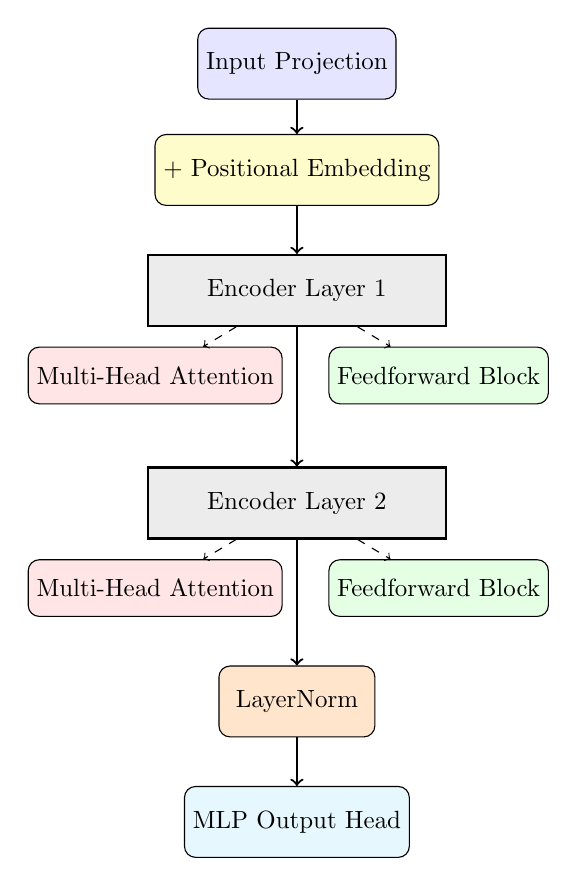
\begin{tikzpicture}[scale=0.9, every node/.style={transform shape}]

        % Input projection
        \node[draw, rounded corners, minimum width=2.5cm, minimum height=1cm, fill=blue!10] (input) at (0,0) {Input Projection};

        % Positional Encoding
        \node[draw, rounded corners, minimum width=2.5cm, minimum height=1cm, fill=yellow!20] (pos) at (0,-1.5) {+ Positional Embedding};

        % Encoder Layer 1
        \node[draw, thick, minimum width=4.2cm, minimum height=1cm, fill=gray!15] (enc1) at (0,-3.2) {Encoder Layer 1};

        % Attention block
        \node[draw, rounded corners, minimum width=2.8cm, minimum height=0.8cm, fill=red!10] (attn1) at (-2,-4.4) {Multi-Head Attention};
        \node[draw, rounded corners, minimum width=2.8cm, minimum height=0.8cm, fill=green!10] (ffn1) at (2,-4.4) {Feedforward Block};

        % Encoder Layer 2
        \node[draw, thick, minimum width=4.2cm, minimum height=1cm, fill=gray!15] (enc2) at (0,-6.2) {Encoder Layer 2};

        \node[draw, rounded corners, minimum width=2.8cm, minimum height=0.8cm, fill=red!10] (attn2) at (-2,-7.4) {Multi-Head Attention};
        \node[draw, rounded corners, minimum width=2.8cm, minimum height=0.8cm, fill=green!10] (ffn2) at (2,-7.4) {Feedforward Block};

        % Normalisation
        \node[draw, minimum width=2.2cm, minimum height=1cm, fill=orange!20, rounded corners] (norm) at (0,-9) {LayerNorm};

        % Output head
        \node[draw, minimum width=2.8cm, minimum height=1cm, fill=cyan!10, rounded corners] (output) at (0,-10.7) {MLP Output Head};

        % Arrows
        \draw[->, thick] (input) -- (pos);
        \draw[->, thick] (pos) -- (enc1);
        \draw[->, thick] (enc1) -- (enc2);
        \draw[->, thick] (enc2) -- (norm);
        \draw[->, thick] (norm) -- (output);

        % Dashed paths to attention/feedforward
        \draw[->, dashed] (enc1) -- (attn1);
        \draw[->, dashed] (enc1) -- (ffn1);
        \draw[->, dashed] (enc2) -- (attn2);
        \draw[->, dashed] (enc2) -- (ffn2);

    \end{tikzpicture}
    \caption{Architecture of the Transformer encoder used}
    \label{fig:transformer_encoder_diagram}
\end{figure}